\documentclass[conference]{IEEEtran}
\IEEEoverridecommandlockouts
\usepackage{cite}
\usepackage{amsmath,amssymb,amsfonts}
\usepackage{algorithmic}
\usepackage{graphicx}
\usepackage{textcomp}
\usepackage{xcolor}
\usepackage{listings}
\usepackage{pgfplots}
\usepackage{float}
\usepackage{booktabs}
\usepackage{url}
\usepackage{hyperref}
\usepackage{fancyvrb}
\usepackage{caption}
\captionsetup[figure]{justification=centering}
% Add after your package imports, before \begin{document}
\renewcommand{\thefigure}{\arabic{figure}}
\renewcommand{\thetable}{\arabic{table}}
\pgfplotsset{compat=1.18}
\definecolor{bg}{RGB}{255,255,226}
\def\BibTeX{{\rm B\kern-.05em{\sc i\kern-.025em b}\kern-.08em
    T\kern-.1667em\lower.7ex\hbox{E}\kern-.125emX}}

\lstdefinestyle{input}{
    basicstyle=\ttfamily\bfseries,
    backgroundcolor=\color{white},
    frame=none,
    breaklines=true,
    showstringspaces=false,
    xleftmargin=0pt,
    xrightmargin=0pt
}

\begin{document}

\title{Pizzeria Scheduler Report}
\author{Daniel A. Marin}
\date{\today}

\maketitle

\begin{abstract}
    This report presents a simulation of a pizza scheduling system that leverages various scheduling algorithms to optimize the process of pizza preparation, baking, and delivery. The project demonstrates concepts of operating systems applied in a practical scenario, where order processing and resource allocation are managed using scheduling strategies. The simulation highlights the performance differences between the algorithms. Additionally, the extra credit implementation explores multi-threaded synchronization across multiple restaurant simulations using Java's threading libraries, thereby illustrating practical applications of concurrency control in real-world systems.
\end{abstract}

\section{Introduction}
Scheduling and Synchronization are often overlooked in the world of computer science and software engineering, since they are almost a given by all the operating systems and libraries that we use. However, they play a crucial role in the performance of our applications, especially when dealing with real-time systems or high-performance computing. This project aims to explore the scheduling and synchronization of a simple pizza delivery system, as to gain practical insights into process management, threads, process control, and other related topics. 

This assignment focuses on simulating an assembly line for pizza preparation, baking, and delivery. It models pizza preparation, baking, and delivery through classes that represent ovens, chefs, and drivers, each with configurable constraints. Users can run different scheduling algorithms (e.g., Round Robin, Focused) to compare performance metrics. This document explains the overall system design, provides instructions for building and testing the application, and includes sample outputs from representative runs.

\subsection{Objective}
The objectives of this project are the following:
\begin{itemize}
    \item Obtain in-depth understanding of process management, threads, multithreading, remote process-call and communication.
    \item Construct a program module for an operating system that simulates a pizza delivery system.
    \item Become proficient system programmers.
\end{itemize}


\subsection{Problem Statement}
This assignment aims to simulate a pizza delivery system. The system consists of a pizza shop, which only produces Hawaiian Pizza, that receives a set of orders from customers (via. a `txt' file). The program needs to prepare, cook and deliver the pizzas to the customers. 

\subsection{Compile and Run Instructions}
The project is written in Java and can be compiled and run using a Shell Script provided for both Windows and MacOS. The shell script is located in the \textit{Application} folder of the project. 

In MacOS the shell script can be run by executing the following commands in the terminal: \texttt{cd Application}, \texttt{chmod +x Shell.sh} and \texttt{./Shell.sh}. The shell script will prompt the user to enter the desired configuration for the simulation. To compile it use the following command: \texttt{./Shell.sh compile}, for unit testing use: \texttt{./Shell.sh test}, and for a manual on predetermined configurations write \texttt{./Shell.sh help}.

In Windows the shell script can be run by executing the following commands in the terminal: \texttt{cd Application}, \texttt{.$\backslash$Shell.bat}. The shell script will prompt the user to enter the desired configuration for the simulation. To compile it use the following command: \texttt{.$\backslash$Shell.bat compile}, for unit testing use: \texttt{.$\backslash$Shell.bat test}, and for a manual on predetermined configurations write \texttt{.$\backslash$Shell.bat help}.

For, the purpose of this report, the shell script will be used to run the simulations and the configurations will be explained in the Methodology section. A run-time demo is provided in \href{https://www.youtube.com/watch?v=QjEa1RC2i9c}{Run-time Demo}.

\section{Methodology}
\subsection{Development Environment}
The project was developed using the Java programming language and the VSCode IDE. It requires a Java Development Kit (JDK) to be preinstalled on the system. The class diagram was created using Lucidchart for visualization purposes.

\subsection{System Design}
The system design of this project can be broken down into multiple components: chefs, ovens, drivers, orders, schedulers, simulations, and the main program. Each component plays a specific role in accomplishing the task of preparing and delivering Hawaiian Pizzas. The following class diagram illustrates the relationships and the classes that make up the system:


\begin{figure*}[ht]
    \centering
    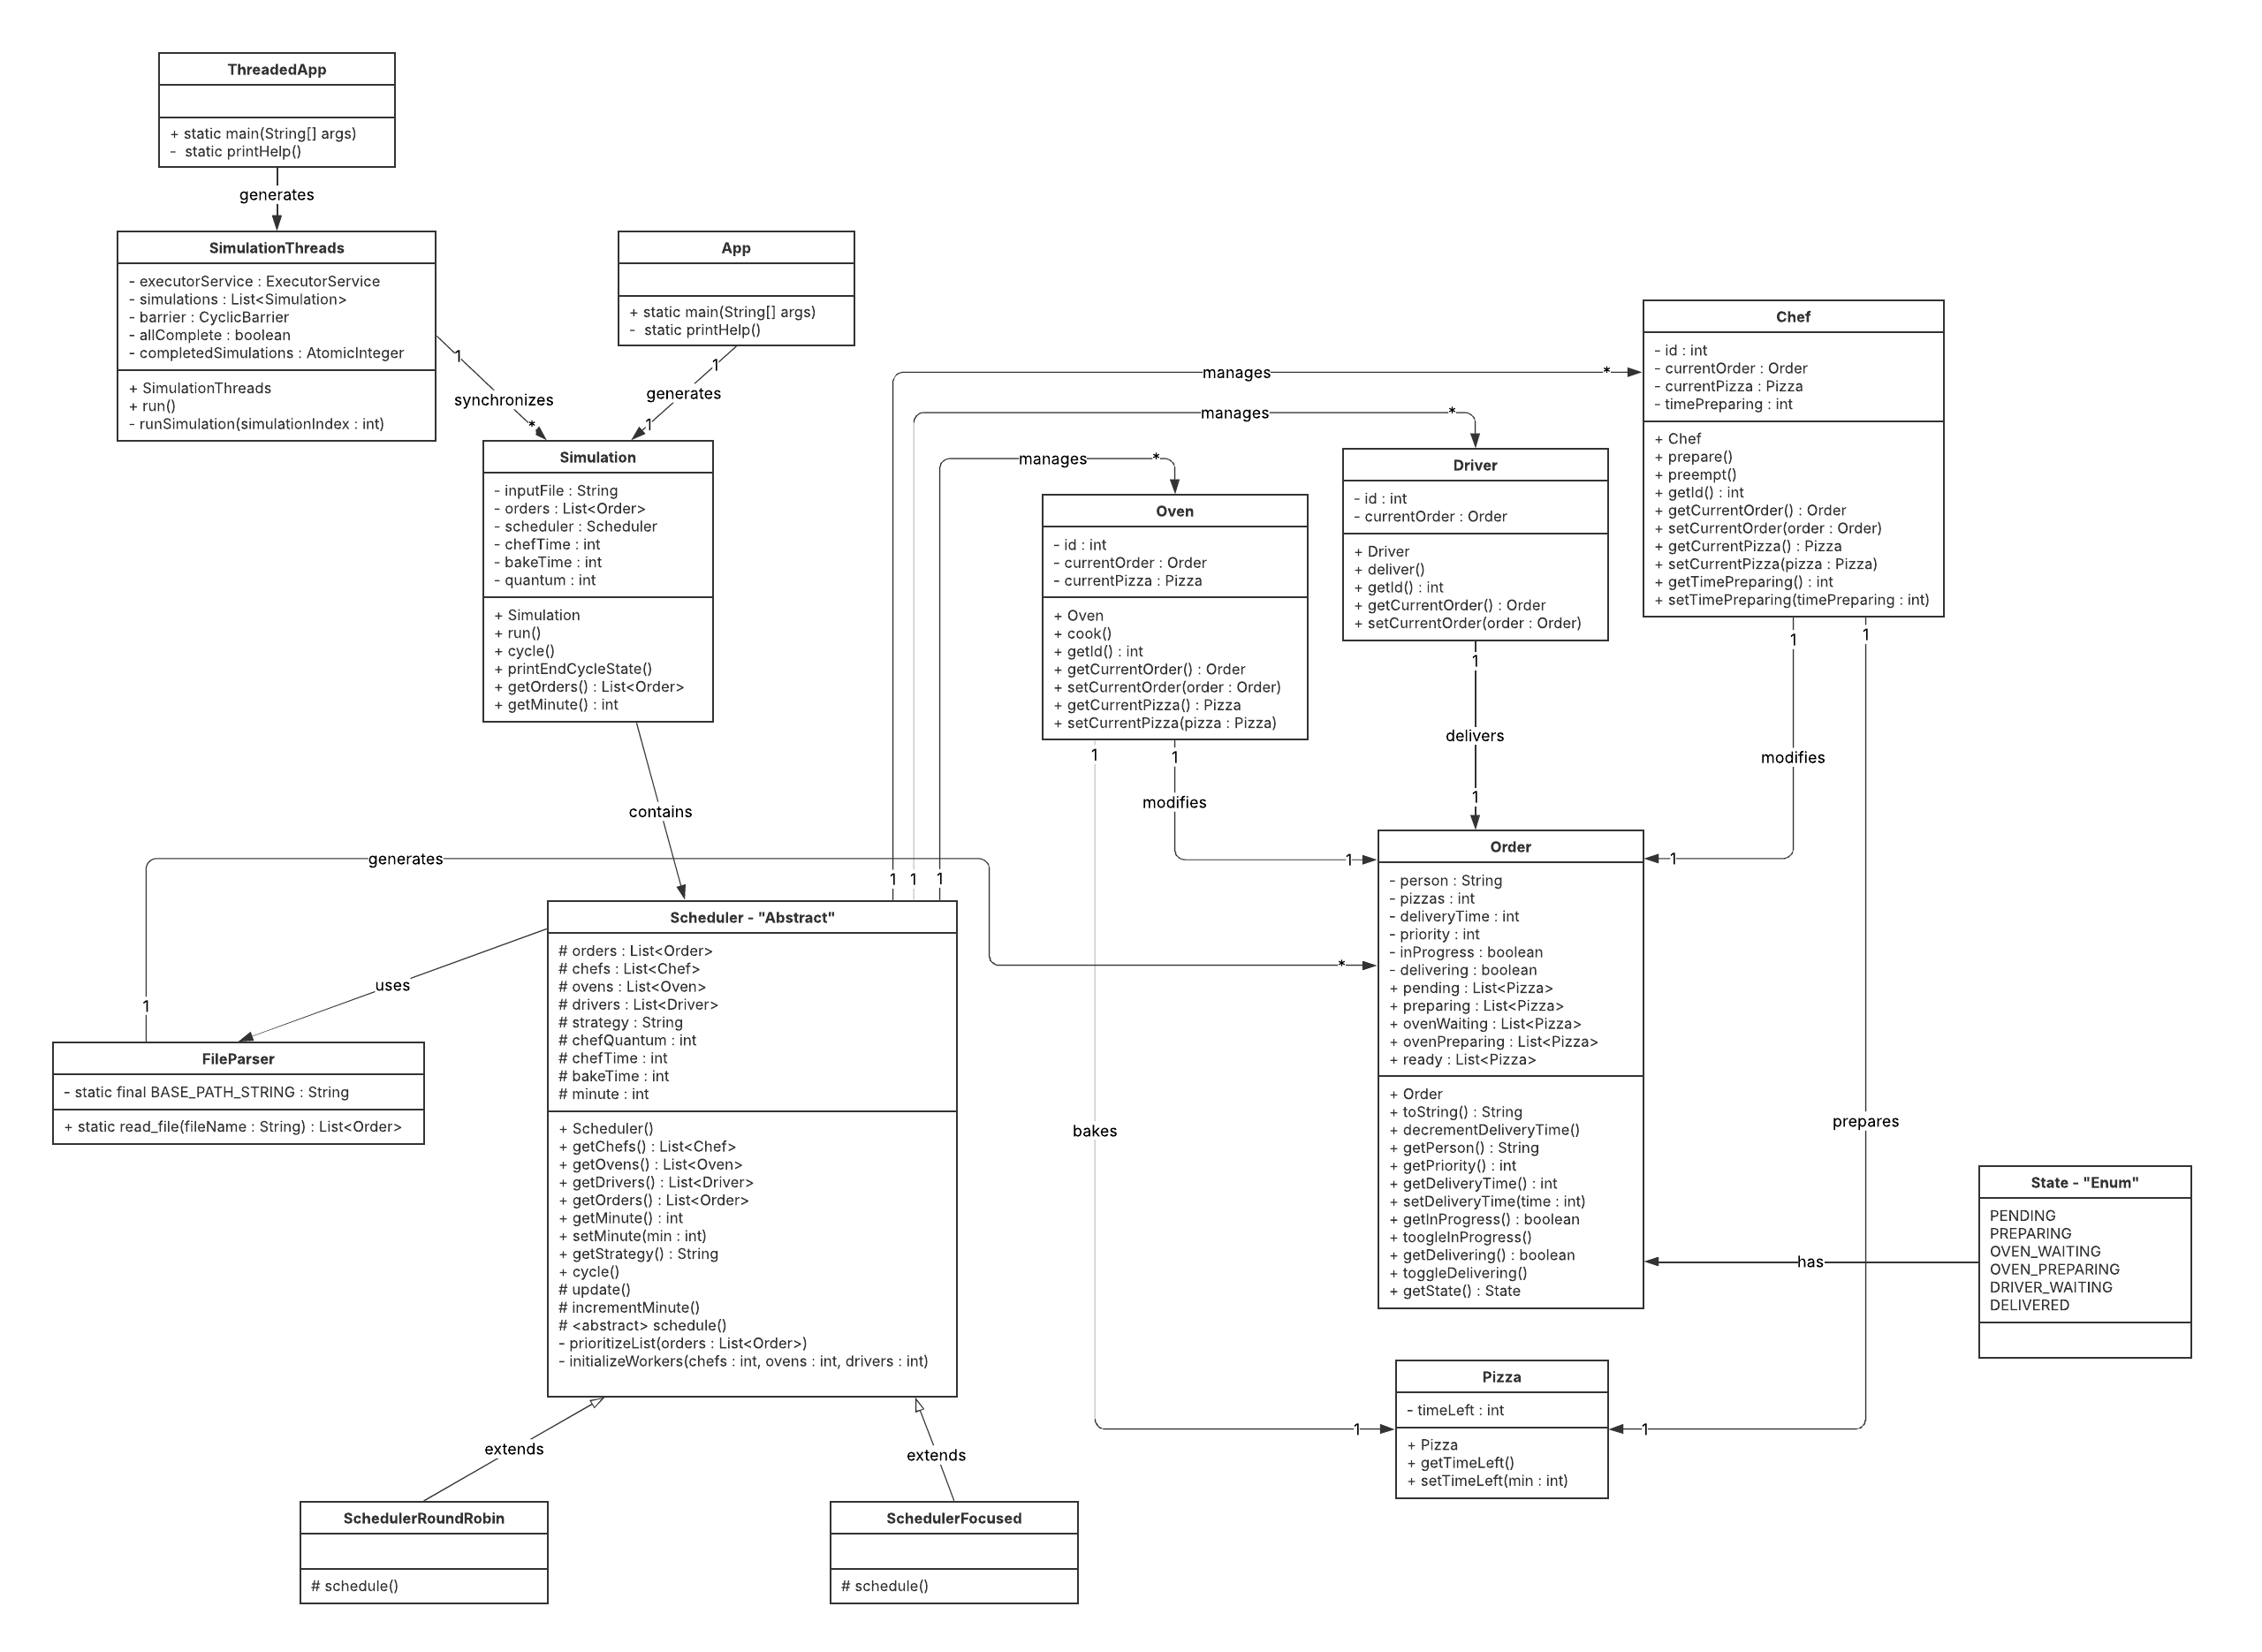
\includegraphics[width=\textwidth]{ClassDiagram.png}
    \caption{\centering Class Diagram for Pizzeria Simulation System}
    \label{fig:class_diagram}
\end{figure*}

As we can visualize in Fig. \ref{fig:class_diagram}, all the components are interconnected and work together to simulate the pizza delivery system. The main program is responsible for reading the orders from a file, and initializing a simulation with the specified configuration. The simulation is responsible for determining the correct scheduler, which then manages the preparation of the orders with the use of the system resources (chefs, ovens, and drivers). The resources are then the ones responsible for processing the pizzas and updating the orders accordingly. 

\subsection{System Components}
The system is composed of the following components: chefs, ovens, drivers, orders, scheduler, and simulation. Each component has a specific role in the system. The chefs, ovens, and drivers represent resources that are scheduled by the scheduler. The orders are read from a file and are processed based on their priority number. The simulation runs until all the orders have been processed.

\subsubsection{Resources}
The chefs, ovens, and drivers represent resources in a fashion similar to a CPU in an operating system. The scheduling configuration for each resource can be specified by the user. 

Chefs are responsible for preparing the pizzas. They can work in two modes: focused mode and round-robin mode. In focused mode, chefs work on one pizza at a time until completion before moving on to the next pizza (First-come First-serve with no preemption). In round-robin mode, chefs work on a pizza for a specified time quantum before moving on to the next pizza (Round-robin with preemption); round-robin requires a \textit{working} time quantum to be specified. These modes represent different scheduling algorithms used by operating system schedulers when handling processes/threads. 

Ovens are responsible for baking the pizzas. They can only work in focused mode (First-come First-serve with no preemption), as it is ill-advised to interrupt the baking process once it has started. 

Drivers are responsible for delivering the pizzas. They only work in focused mode (First-come First-serve with no preemption); drivers deliver orders instead of pizzas and can only deliver one order at a time.

\subsubsection{Orders}
Orders are read from a file and are processed based on their priority number. The lower the number, the higher the priority. Orders have a specified delivery time, which is the time it takes to deliver the order once it has been prepared and baked. They also have a state that represents the current status of the order (e.g., waiting, preparing, baking, delivering).

\subsection{Scheduling Algorithms}
The scheduling algorithms used in this project are the following:
\begin{enumerate}
    \item Priority-based Scheduling (Order): priority based scheduling is used to determine the sequence in which orders are processed. The lower the priority number, the higher the priority. This is acheived by sorting the orders based on their priority number, using the priority queue data structure from the Java Utility library. Resource are allocated to the orders based on the order of the priority queue.
    \item Round-robin Scheduling (Chef): round-robin scheduling is used to determine the sequence in which chefs may prepare pizzas. Chefs work on a pizza for a specified time quantum before being `preempted' and moving on to the next pizza. This is acheived by using a queue data structure to store the pizzas that are being prepared by the chefs, and simply popping and pushing pizzas from the queue based on the time quantum.
    \item Focused Scheduling (Chef, Oven, Driver): focused scheduling is used to determine the sequence in which ovens bake, drivers deliver and chefs may prepare pizzas. The concept of this is that any of these resources may only focus on one pizza at a time and they must see through the entire process. Again this is acheived by using a queue data structure to store the pizzas. 
\end{enumerate}

The priority-based scheduling is in charge of managing how orders get processed, meanwhile the round-robin and focused scheduling are in charge of managing how the resources are allocated to the orders. 

\subsection{Test Setup}
\subsubsection{Test Case 1}
This test case is based on scenarios discussed during class, where we wanted to visualize the differences between the Round Robin and the Focused Scheduling algorithms. The configurations for this test cases are as follows:
\begin{enumerate}
    \item Round Robin Scenario (Shell Script: \texttt{./Shell.sh classRR})
    \begin{itemize}
        \item \texttt{--input-file ClassTest.txt}
        \item \texttt{--available-ovens 2}
        \item \texttt{--available-chefs 2} 
        \item \texttt{--available-drivers 2}
        \item \texttt{--bake-time 3}
        \item \texttt{--chef-time 3}
        \item \texttt{--chef-strategy RR}
        \item \texttt{--chef-quantum 1}
    \end{itemize}
    \item Focused Scenario (Shell Script: \texttt{./Shell.sh classFoc})
    \begin{itemize}
        \item \texttt{--input-file ClassTest.txt}
        \item \texttt{--available-ovens 2}
        \item \texttt{--available-chefs 2} 
        \item \texttt{--available-drivers 2}
        \item \texttt{--bake-time 3}
        \item \texttt{--chef-time 3}
        \item \texttt{--chef-strategy FOCUSED}
    \end{itemize}
\end{enumerate}

Where the \texttt{ClassTest.txt} file contains the following orders:
\begin{figure}[H]
    \centering
    \begin{lstlisting}[style=input,frame=single]
Juan,3,1,2
Pedro,1,1,0
    \end{lstlisting}
    \caption{\centering \texttt{ClassTest.txt} file contents}
    \label{fig:orders}
\end{figure}

The reason for this configuration is to visualize the differences in outputs between the two scheduling algorithms. It is expected that the Round Robin and Focused Scheduling algorithms will complete the orders at the same time, but the order in which the pizzas are prepared, baked, and delivered will be different. 

This is because the Round Robin algorithm will switch between pizzas every time quantum, meanwhile the Focused algorithm will see through the entire process of one pizza before moving on to the next one. Due, to the time quantum being the same as a cycle time, the Round Robin algorithm will behave similarly to the Focused algorithm in this case. 

The purpose of this test is to visualize the correctness of the outputs and the differences of each scheduling algorithm.

\subsubsection{Test Case 2}
This test case is based on a scenarios where we wanted to visualize the advantage of the Round-Robin algorithm over the Focused algorithm. For the outputs to be different, the time quantum must be greater than the cycle time and the number of pizzas must be greater than the number of resources. The configurations for this test cases are as follows:
\begin{enumerate}
    \item Round Robin Scenario (Shell Script: \texttt{./Shell.sh five})
    \begin{itemize}
        \item \texttt{--input-file BasicFocused.txt}
        \item \texttt{--available-ovens 2}
        \item \texttt{--available-chefs 2} 
        \item \texttt{--available-drivers 2}
        \item \texttt{--bake-time 6}
        \item \texttt{--chef-time 4}
        \item \texttt{--chef-strategy RR}
        \item \texttt{--chef-quantum 2}
    \end{itemize}
    \item Focused Scenario (Shell Script: \texttt{./Shell.sh one})
    \begin{itemize}
        \item \texttt{--input-file BasicFocused.txt}
        \item \texttt{--available-ovens 2}
        \item \texttt{--available-chefs 2} 
        \item \texttt{--available-drivers 2}
        \item \texttt{--bake-time 6}
        \item \texttt{--chef-time 4}
        \item \texttt{--chef-strategy FOCUSED}
    \end{itemize}
\end{enumerate}

Where the \texttt{BasicFocused.txt} file contains the following orders:
\begin{figure}[H]
    \centering
    \begin{lstlisting}[style=input, frame=single]
John,1,20,1
Maria,3,10,0
    \end{lstlisting}
    \caption{\centering \texttt{BasicFocused.txt} file contents}
    \label{fig:orders1}
\end{figure}

This configuration will lead to the Round Robin algorithm to complete the preparation of the pizzas faster than the Focused algorithm, since one pizza in Maria's order will see progress every time quantum thus leading the preparation of Maria's order to take $6$ time units instead of the $8$ time units that the Focused algorithm will take.
\section{Results}
To perform the scenarios in test case 1 and test case 2, the following shell scripts were used: \texttt{./Shell.sh classRR} and \texttt{./Shell.sh classFoc} for test case 1, and \texttt{./Shell.sh five} and \texttt{./Shell.sh one} for test case 2. The outputs will not be shown in this document, but they can be found in the \texttt{Application/Document/Output} folder of the project as \textit{classRR.txt}, \textit{classFoc.txt}, \textit{five.txt}, and \textit{one.txt}, this decision was performed to reduce the length of this document. 

The outputs in the files are as expected, the Round Robin algorithm completes the orders faster than the Focused algorithm in test case $2$, and the Round Robin and Focused algorithms complete the orders at the same time in test case $1$. Also, it is important to note that the outputs present the correct information of both the orders and the resources.

Examples of how orders are presented are: 
\begin{figure}[H]
    \centering
    \begin{lstlisting}[style=input, frame=single]
> Maria,PREPARING,0,3,10
> John,PENDING,0,1,4
    \end{lstlisting}
    \caption{\centering Order Output}
    \label{fig:order_output}
\end{figure}

Where the output shows the name of the customer, the state of the order, the number of completed pizzas for that state, the number of pizzas that are in progress for that state, and the time remaining for that state to be finished.

Examples of how resources are presented are:
\begin{figure}[H]
    \centering
    \begin{lstlisting}[style=input, frame=single]
> Chef0,Maria
> Chef0,Maria,1
    \end{lstlisting}
    \caption{\centering Order Output}
    \label{fig:res_output}
\end{figure}
 
The output presents the name of the resource, its index, and the name of the order that it is working on (if any) or none; and the time quantum that the resource has left to prepare the pizza if it is in Round Robin mode.

A single cycle is presented as follows:
\begin{figure}[H]
    \centering
    \begin{lstlisting}[style=input, frame=single]
==== Minute 1
Pedro,PREPARING,0,1,2
Juan,PREPARING,0,3,8
Chef0,Pedro
Chef1,Juan
Oven0,None
Oven1,None
Driver0,None
Driver1,None
    \end{lstlisting}
    \caption{\centering Cycle Output}
    \label{fig:cycle_output}
\end{figure}

The results of the test cases show that the system is working as expected and that the scheduling algorithms are correctly implemented.

\section{Conclusion}
This project successfully demonstrates how scheduling and synchronization concepts can be applied to a practical scenario of pizza orders. By modeling chefs, ovens, drivers, and different scheduling strategies, we have verified that Round Robin and Focused Scheduling behave as expected. The simulation results confirm that Round Robin can deliver higher throughput when multiple resources and a time slice are configured, while Focused Scheduling processes each order straight through. The insights gained from this assignment provide us with an understanding of important OS principles in a real-world scenario, underlining the significance of careful resource management and concurrency control.

\appendix
\section{Appendix}
\subsection{Extra Credit}
This section in the Appendix contains the extra credit portion of the assignment. It contains an explanation of the logic behind the synchronization of the multiple restaurants when accessing the shared resource (\texttt{stdout}).

The extra credit portion of this assignment was to implement a system that could handle multiple restaurants as threads and synchronize the access to the shared resource (\texttt{stdout}). The implementation of this system was done by creating a \texttt{SimulationThreads} class that utilizes the \textit{ExecutorService}, \textit{CyclicBarrier}, and \textit{AtomicInteger} classes from the Java Utility library, to synchronize the printing of each cycle for multiple simulations. 

The \texttt{SimulationThreads} class is responsible for creating the instances of each simulation and assigning them to an \textit{ExecutorService} thread pool. The \textit{ExecutorService} thread pool is responsible for executing the simulations for each restaurant. The \textit{CyclicBarrier} class is used to synchronize the printing of each cycle for multiple simulations, as each thread must wait for all threads to complete their current cycle before printing. The \textit{AtomicInteger} class is used to keep track of the number of simulations that have been completed.

The barrier provides a synchronization point for the threads and single access to the critical section of this program, which is the printing of a cycle. Meanwhile, the AtomicInteger provides control over when to end the entire simulation, as it keeps track of the number of simulations that have been completed.

To test out this, we created a test case that simulates the behavior of multiple restaurants. The test case is as follows - Multiple Restaurants Scenario (Shell Script: \texttt{./Shell.sh three}):
\begin{itemize}
    \item \texttt{--input-file BasicFocused.txt,BasicRo-
    undRobin.txt}
    \item \texttt{--available-ovens 2}
    \item \texttt{--available-chefs 2} 
    \item \texttt{--available-drivers 2}
    \item \texttt{--bake-time 6}
    \item \texttt{--chef-time 4}
    \item \texttt{--chef-strategy FOCUSED}
\end{itemize}

Where the \texttt{BasicFocused.txt} file contains the following orders:
\begin{figure}[H]
    \centering
    \begin{lstlisting}[style=input, frame=single]
John,1,20,1
Maria,3,10,0
    \end{lstlisting}
    \caption{\centering \texttt{BasicFocused.txt} file contents}
    \label{fig:orders2}
\end{figure}

And the \texttt{BasicRoundRobin.txt} file contains the following orders:
\begin{figure}[H]
    \centering
    \begin{lstlisting}[style=input, frame=single]
Maria,3,10,0
    \end{lstlisting}
    \caption{\centering \texttt{BasicRoundRobin.txt} file contents}
    \label{fig:orders3}
\end{figure}

The purpose of this test case is to visualize the synchronization of the printing of each cycle for multiple simulations. To compare this with the single threaded version of this simulation, the \texttt{./Shell.sh one} command can be used to run the same configuration with input file \texttt{BasicFocused.txt}; and the \texttt{./Shell.sh two} command can be used to run the same configuration with input file \texttt{BasicRoundRobin.txt}.

Again, the results of this test case will not be shown in this document, but they can be found in the \texttt{Application/Document/Output} folder of the project as \textit{three.txt}, \textit{second.txt},and \textit{one.txt}, this decision was performed to reduce the length of this document.

The contents of the output files are as expected, synchronization of the printing does take place since both restaurants are allowed to print their correct state of the orders concurrently, while executing in parallel. The results of running \texttt{./Shell.sh three} present the same state of all simulation than those same simulations running by themselves. Thus, the synchronization and threading of the printing is successful. 
\end{document}